\documentclass[titlepage]{article}
\usepackage[utf8]{inputenc}
\usepackage{hyperref}
\usepackage{float}
\restylefloat{figure}
\usepackage{subcaption}
\usepackage{amsmath}
\usepackage{amssymb}
\usepackage{minted}
\usepackage{graphicx}
\DeclareGraphicsExtensions{.eps}
\usepackage{fancyhdr}
\pagestyle{fancy}
\lhead{Fractals and the Beauty of Nature}
\author{Chanthosh Sivanandam \\ Erik Andersen \\ Henrik Flindt }
\title{Fractals and the Beauty of Nature \\ DM550 - Fall Project 2017}
\begin{document}
\maketitle
\section{Sierpinski Triangle}
Initially, implementation of the Sierpinski triangle was build upon the idea of placing inverted triangles inside other triangles. It turned out to be a tad complicated, but it yielded some rather interesting results, which can be seen here:
\begin{figure}[H]
  \centering
  \begin{subfigure}[b]{0.4\textwidth}
    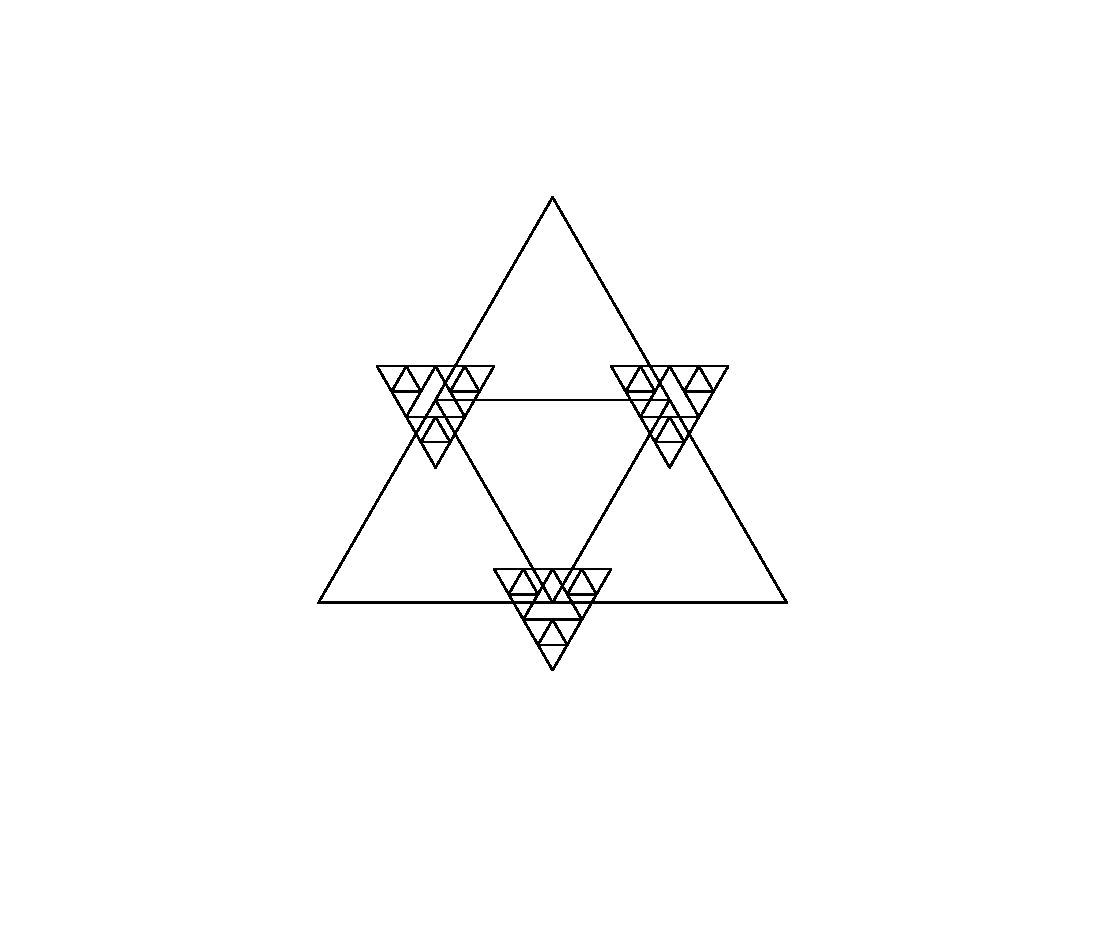
\includegraphics[width=\textwidth]{wrongtriangle}
    \caption{An unsuccessful attempt}
  \end{subfigure}
  \begin{subfigure}[b]{0.5\textwidth}
    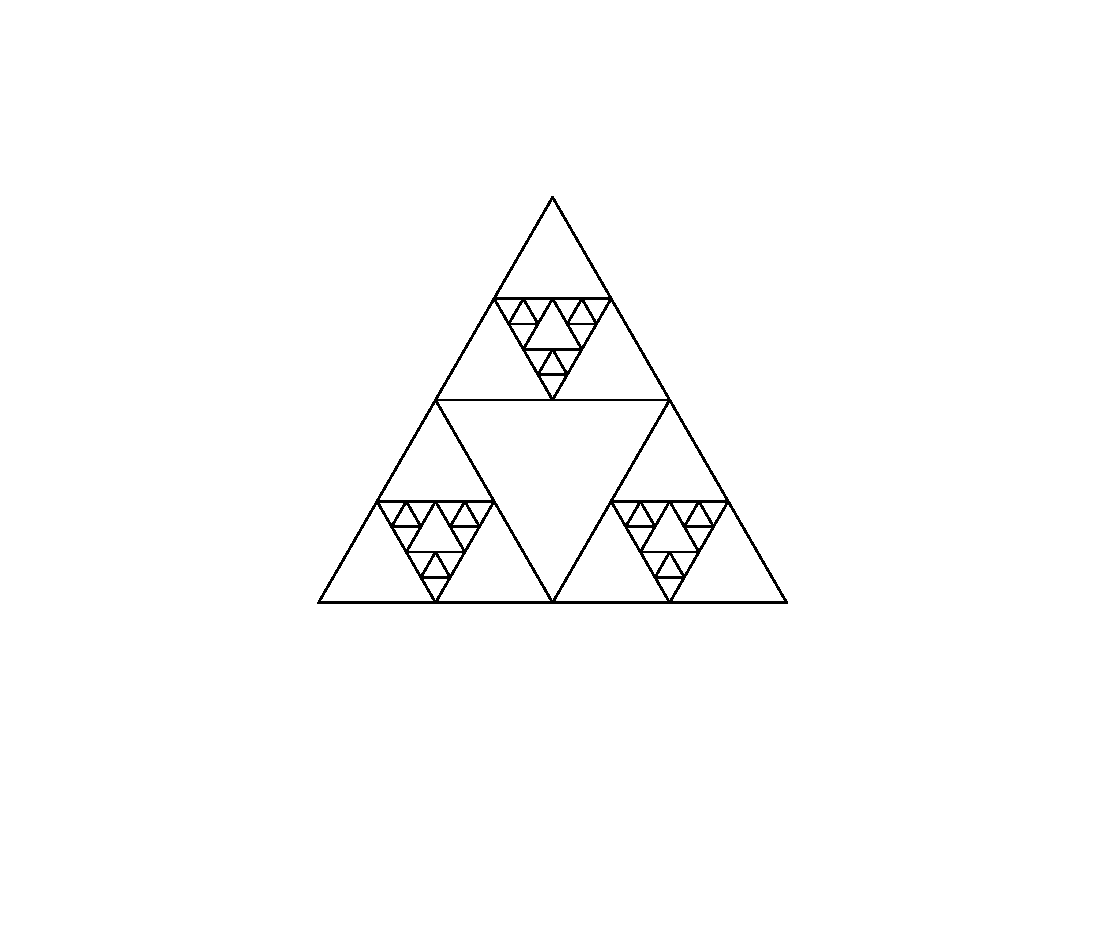
\includegraphics[width=\textwidth]{wrongtriangle2}
    \caption{Another unsuccessful attempt}
  \end{subfigure}
\end{figure}
After meddling around for some time, a decision was made to try the approach suggested in the project description. A successful algorithm that gave the expected result was then rapidly developed.
\begin{figure}[H]
  
\includegraphics[width=0.6\textwidth]{triangle}
  \caption{Sierpinski triangle with 5 subdivisions.}
\end{figure}
Revisiting the initial code, the faultiness of its algorithm became apparent and hence could be corrected. The effectiveness of this new code compared to the approach recommended in the project description is due to the lack of redundant drawing. \par We used an iterative development process, meaning we started out by making a small piece of the code work in one iteration. Through testing, trial and error the goal of the iterative step was reached and we then carried on with the next step, where more code was implemented and tested. After several steps, we realized that our approach was overly complicated, so we started again from scratch. This time we did not care for optimization of the algorithm, and we solely focused on correctness.\footnote{The source code for this part of the project can be found in the file \href{https://github.com/ErikAndersen81/DM550-FractalProject/blob/master/sierpinsky-triangle.py}{sierpinsky-triangle.py}}
\begin{figure}[H]
  \centering
  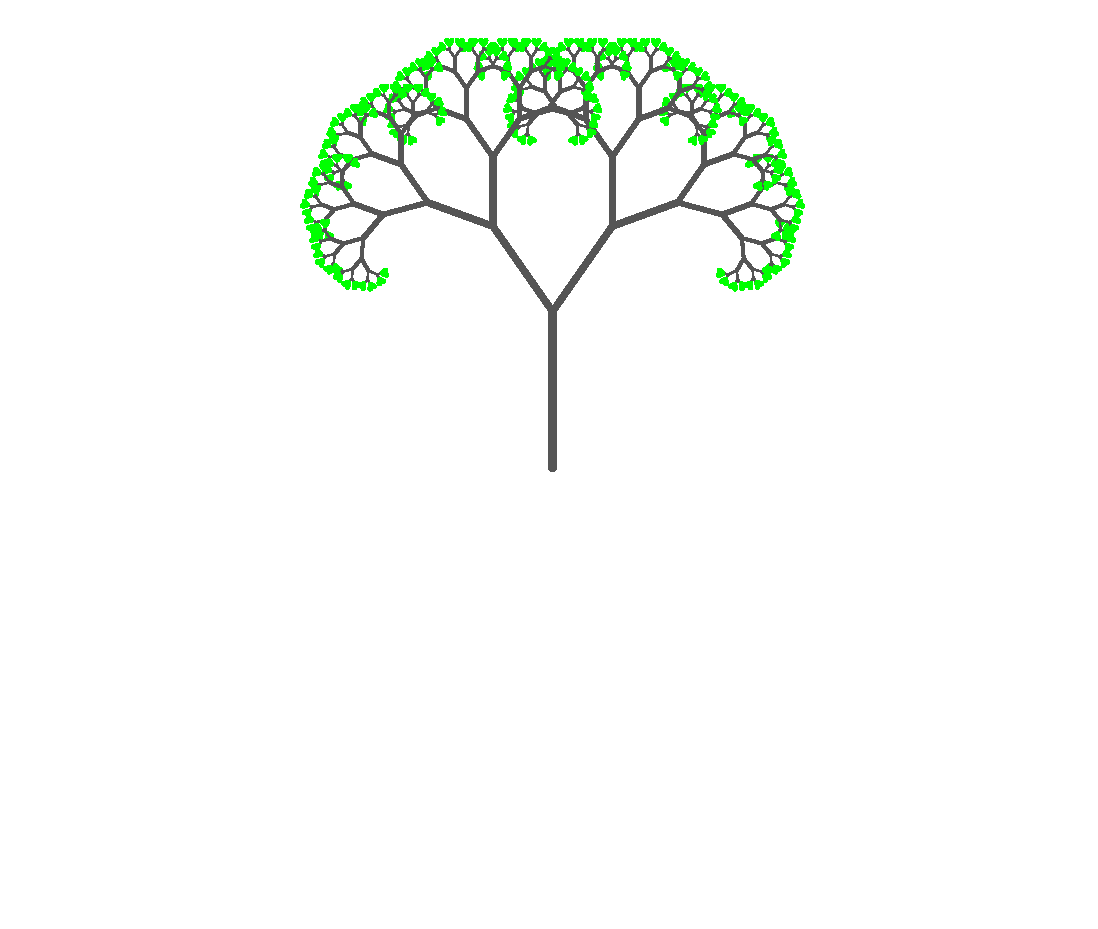
\includegraphics{bintree}
  \caption{Binary tree}
\end{figure}
section{Binary three}
\subsection{Specification and design}
We began by trying to define a function with two parameters (size, step)
\end{document}
